% Chapter 2 (from main tex file)
% Research Project
% Author: Javier Reyes

% TODO: Complete chapter

\chapter{Hardware Platform Design}

The workflow for the Zynq-7000 architecture starts with the hardware specification for both PS and PL technologies. Xilinx provide a complete suite of programs and tools for the entire desing cycle of the embedded solution, either in a standalone platform or in an embedded OS.

\begin{figure}[htp]
	\centering
	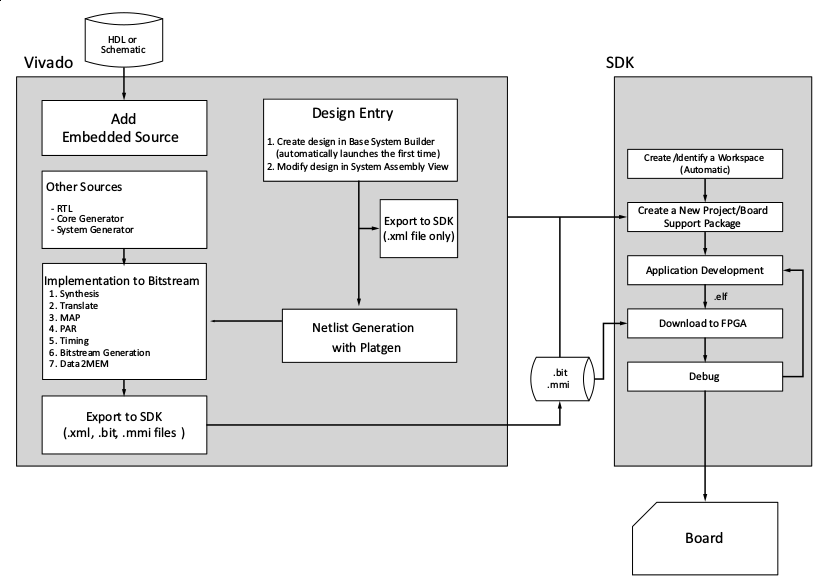
\includegraphics[width=\textwidth]{embedded-flow.png}
	\caption{Embedded Design Process Flow, from \cite{UG1043}.} \label{fig:embedded-flow}
\end{figure}%

The workflow is split into different tools provided by Xilinx. The hardware specific tasks will be covered in section \ref{hardware-design}. The software component will be covered in chapters \ref{embedded-linux} and \ref{software-application}.

\section{Hardware Design} \label{hardware-design}

For the definition, configuration and flashing of the FPGA fabric, the Vivado Design Suite includes the necessary tools. The 

\subsection{Vivado GUI}

\subsection{TCL Console}

\subsection{Block Design}

\subsection{IP Core}

\subsection{High Level Synthesis}
